\documentclass[a4paper,12pt]{article}
\usepackage[slovene]{babel}
\usepackage[utf8]{inputenc}
\usepackage[T1]{fontenc}
\usepackage[a4paper, total={16cm, 22cm}]{geometry}
\usepackage{lmodern}
\usepackage{amsmath,amsfonts}
\usepackage{amsthm}
\usepackage{setspace}
\usepackage[shortlabels]{enumitem}
\usepackage{graphicx}
\usepackage{float}


\def\N{\mathbb{N}}
\def\Z{\mathbb{Z}}
\def\Q{\mathbb{Q}}
\def\R{\mathbb{R}}

\theoremstyle{definition}
\newtheorem{definicija}{Definicija}
\newtheorem{zgled}{Zgled}
\theoremstyle{plain}
\newtheorem{izrek}{Izrek}
\newtheorem{lema}{Lema}

\newcommand{\inner}[2]{\langle{#1},{#2}\rangle}

\DeclareMathOperator*{\SE}{SE}
\DeclareMathOperator*{\IQR}{IQR}
\DeclareMathOperator*{\IZ}{IZ}
\DeclareMathOperator*{\E}{E}
\DeclareMathOperator*{\Var}{Var}
\DeclareMathOperator*{\Lin}{Lin}
\DeclareMathOperator*{\im}{Im}
\DeclareMathOperator*{\Fisher}{Fisher}

\newenvironment{dokaz}{\begin{proof}[\bfseries\upshape\proofname]}{\end{proof}}

\newcommand{\geslo}[2]{\noindent \textbf{#1} \quad #2 \hfill \break}

\setstretch{1.2}

\title{Projektna naloga pri statistiki}
\author{Matevž Miščič}



\begin{document}

\maketitle{}

\section{Kibergrad}

Pri tej nalogi bomo uporabili program \textbf{kibergrad.py}. Ta program prikaže oba grafikona z intervali zaupanja. Izhod tega programa je zapisan pri vsaki podnalogi posebej v okolju \verb+verbatim+.

\begin{enumerate}[a)]
    \item Na podlagi enostavnega slučajnega vzorca $200$ družin moramo oceniti povprečno število otrok na družino $\mu$. Označimo z $X_i$ število otrok v $i$-ti družini iz vzorca. Cenilka za povprečno število otrok $\mu$ na celi populaciji je kar povprečje na vzorcu $\widehat{\mu} = \overline{X}$. Kot vrne program je povprečje na vzorcu enako $1.02$.
    
    \begin{verbatim}
Povprečje na vzorcu je 1.02.
    \end{verbatim}
    
    \item Standardno napako bomo ocenili s pomočjo nepristranske cenilke 
    $$\widehat{\SE}_{+}^2 = \frac{N - n}{Nn(n - 1)}\sum_{i = 1}^n (X_i - \overline{X})^2,$$ kjer je $N$ število vseh družin, $n$ število družin v vzorcu, $X_i$ število otrok v $i$-ti družini vzorca in $\overline{X}$ povprečje na vzorcu. Kot vrne program je standardna napaka približno enaka $\widehat{\SE}_{+} = 0.08497$.

    Ker je populacija zelo velika, saj vsebuje 43886 družin, bomo predpostavili, da so vrednosti $X_i$ neodvisne. Potem je po centralnem limitnem izreku spremenljivka $\frac{\overline{X} - \mu}{\SE}$ porazdeljena približno standardno normalno, saj je $n = 200$ dokaj veliko število. Recimo tudi, da je $\widehat{\SE}_{+}$ dokaj blizu $SE$ in da je tudi $$\frac{\overline{X} - \mu}{\widehat{\SE}_{+}}$$ porazdeljena približno standardno normalno. Potem lahko dobimo približni interval zaupanja za $\mu$ kot 
    $$\IZ = \left( \overline{X} - c, \overline{X} + c \right), \; \text{ kjer je } c = \widehat{\SE}_{+} \Phi^{-1}\left(1 - \frac{\alpha}{2}\right).$$
    Na podlagi tega dobimo, da je interval zaupanja enak $\IZ = \left( 0.85, 1.19 \right)$

    \begin{verbatim}
Ocena standardne napake je 0.0839710432109479 interval zaupanja 
pa je (0.8554167553065422, 1.1845832446934579).
    \end{verbatim}

    \item Poprečje na celotni populaciji je enako $0.9479$, kar je nekoliko manj kot ocena, ki smo jo dobili iz enostavnega slučajnego vzorca. Prava standardna napaka je enaka $0.08180$, torej je ocena za standardno napako, ki smo jo dobili iz slučajnega vzorca, blizu pravi vrednosti. Vidimo tudi, da interval zaupanja $\IZ$, ki smo ga izračunali v prejšnji točki, vsebuje populacijsko povprečje.
    
    \begin{verbatim}
Povprečje celotne populacije je 0.9479332816843641, prava standardna 
napaka pa 0.08179866349073553.
Interval zaupanja vsebuje populacijsko povprečje.
    \end{verbatim}
    
    \item Vzemimo sedaj še $99$ novih enostavnih slučajnih vzorcev. Intervali zaupanja od vseh 100 vzorcev so narisani na naslednjem grafikonu. Z oranžno je narisano populacijsko povprečje.
    
    \begin{figure}[H]
        \centering
        \label{fig:iz1}
        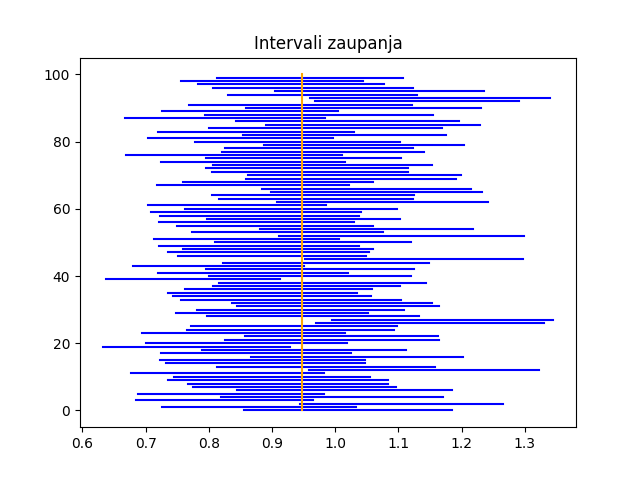
\includegraphics[width=0.7\textwidth]{intervaliZaupanja1.png}
    \end{figure}

    Od vseh $100$ intervalov zaupanja jih $91$ pokrije populacijsko povprečje. Glede na to, da so to $95 \%$ intervali zaupanja, smo pričakovali, da jih bo okoli $95$ vsebovalo populacijsko povprečje, kar se res zgodi.

    \begin{verbatim}
Od 100 intervalov zaupanja jih 91 vsebje populacijsko povprečje.
    \end{verbatim}
    
    \item Standardni odklon za $100$ vzorčnih povprečij je enak $0.085$, standardna napaka za prvotni vzorec velikosti $200$ pa je $0.084$. Obe vrednosti sta si podobni.

    \begin{verbatim}
Standardna napaka vzorca je 0.0839710432109479, 
standardni odklon pa je 0.08526259437760499.
    \end{verbatim}
    
    \item Vzemimo še $100$ enostavnih slučajnih vzorcev velikosti $800$. Za vsakega določimo $95 \%$ interval zaupanja. Intervali so prikazani na spodnji sliki.
    
    \begin{figure}[H]
        \centering
        \label{fig:iz2}
        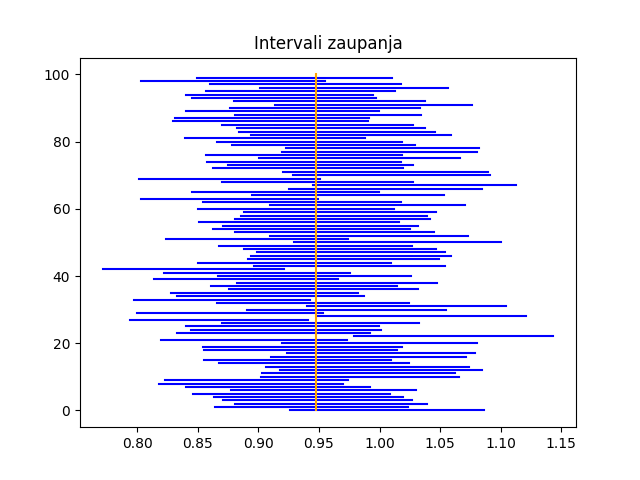
\includegraphics[width=0.7\textwidth]{intervaliZaupanja2.png}
    \end{figure}

    Tokrat $95$ od vseh $100$ intervalov zaupanja pokrije populacijsko povprečje.
    Standardni odklon vzočnih povprečij je tokrat $0.0403$, stadnardna napaka pa je $0.0410$. Vrednosti sta si spet podobni.

    Opazimo lahko, da je na večjih vzorcih standardna napaka manjša. Poleg tega so intervali zaupanja krajši čeprav so še vedno $95 \%$.

    \begin{verbatim}
Od 100 intervalov zaupanja jih tokrat 95 vsebje populacijsko 
povprečje.
Standardna napaka vzorca je 0.04100979217200208, 
standardni odklon pa je 0.040326402641445706.
    \end{verbatim}
\end{enumerate}


\section{Hobotnice}
V tem nalogi bomo ugotovili, ali so hrbtne dolžine različnih vrst hobotnic približno v skladu z log-normalnim modelom. Naj bo $X$ slučajna spremenljivka, ki je porazdeljena enakomerno na množici podatkov in naj bo $Y = \log{X}$. Če je $X$ res porazdeljena v skladu z log-normalnim modelom, je $Y$ porazdeljena v skladu z normalnim modelom. Pričakovana vrednost $Y$ je enaka $3.51$, standardni odklon pa je $0.78$.

\begin{verbatim}
mi =  3.50827914588622
sigma =  0.7811547435375114
\end{verbatim}

\noindent
Narišimo histogram skupaj z log-normalno gostoto. Najprej moramo določiti širino razreda po modificiranem Freedman–
Diaconisovim pravilu. Širina mora torej biti enaka $$\frac{2.6 \cdot \IQR}{\sqrt[3]n} = 23.016,$$ kjer je $\IQR$ interkvartilni razmik, $n$ pa je število podatkov. 

\begin{verbatim}
Širina razredov hrbtnih dolžin hobotnic po modificiranem 
Freedman-Diaconisovem pravilu je 23.016005260370942.
\end{verbatim}

\noindent
Gostoto log-normalne porazdelitve lahko izračunamo s pomočjo transformacijske formule, sicer pa lahko uporabimo tudi funkcijo \verb+lognorm.pdf()+ iz knjižnice \verb+scipy.stats+.

\begin{figure}[H]
    \centering
    %\caption{Histogram 1}
    \label{fig:hist1}
    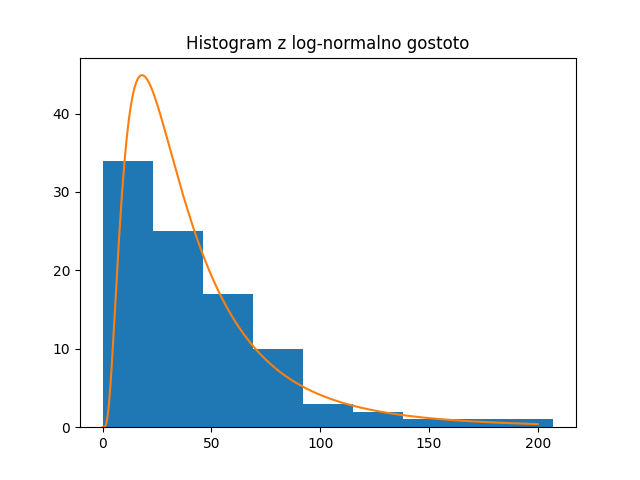
\includegraphics[width=0.7\textwidth]{Histogram1.png}
\end{figure}

Sedaj narišimo še histogram na logaritemski lestvici in dorišimo še ustrezno normalno gostoto. Če uporabimo modificirano Freedman–
Diaconisovo pravilo, da določimo širino razreda desetiških logaritmov, ugotovimo, da morajo biti razredi širine $0.282$. 

\begin{verbatim}
Širina razredov desetiških logaritmov hrbtnih dolžin hobotnic po 
modificiranem Freedman-Diaconisovem pravilu je 0.28238411234417427.
\end{verbatim}

Dobimo naslednji histogram.

\begin{figure}[H]
    \centering
    %\caption{Histogram 2}
    \label{fig:hist2}
    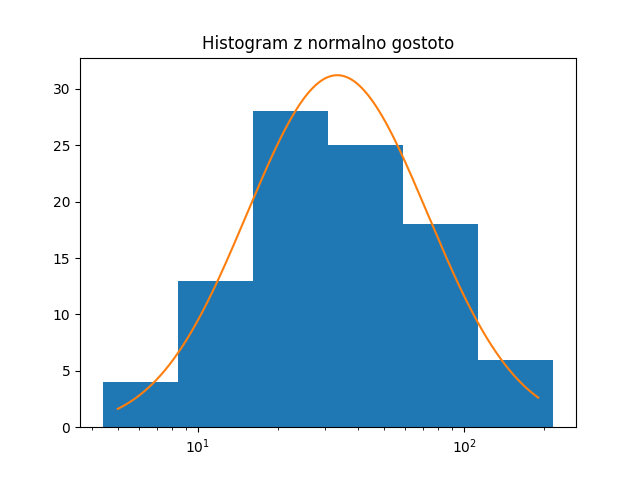
\includegraphics[width=0.7\textwidth]{Histogram2.png}
\end{figure}

Vidimo, da se pri obeh histogramih podatki o hrbtnih dolžinah hobotnic dobro prilegajo ustreznima gostotama.

Nazadnje primerjajmo podatke z log-normalno gostoto še s primerjalnim kvantilnim (Q–Q) grafikonom. Na grafikonu bomo obe osi prikazali na logaritemski lestvici.

\begin{figure}[H]
    \centering
    %\caption{Q-Q grafikon}
    \label{fig:qqgraph}
    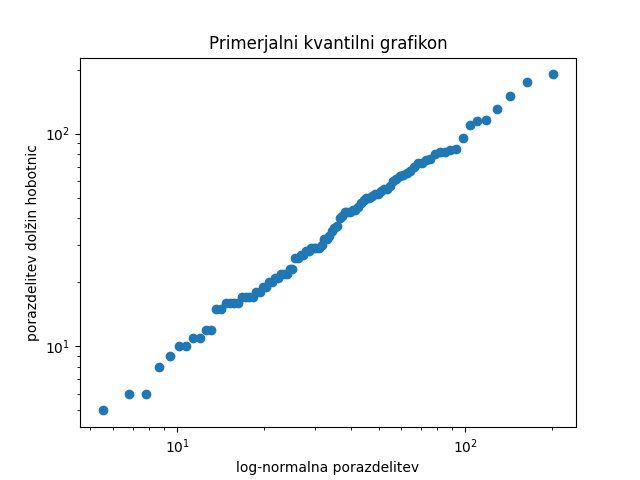
\includegraphics[width=0.7\textwidth]{PrimerjalniGrafikon.png}
\end{figure}

Točke na tem grafikonu ležijo približno na premici. Sklepamo, da so torej podatki res približno v skladu z log-normalnim modelom.

Pri tej nalogi smo uporabljali program \textbf{hobotnice.py}. Ta program zgenerira ob histograma in primerjalni kvantilni grafikon, hkrati pa izpiše izračune, ki so dodani pri vsakem delu naloge.

\section{Piščanci}
Pri tej nalogi bomo ugotovili, kako se spreminja teža piščanca s časom in ali dieta vpliva na pridobivanje teže piščanca.

\begin{enumerate}[a)]
    \item Oceniti moramo, koliko teže piščanec pridobi vsak dan. Za vsakega piščanca privzemimo, da pridobiva težo po statističnem modelu $Y_i = a + b X_i + \epsilon_i$, kjer je $Y_i$ masa piščanca v gramih $X_i$ dni po rojstvu, $\epsilon_i$ pa predstavlja šum. Privzemimo, da za vsak $i$ velja $\E(\epsilon_i) = 0$, $\Var(\epsilon_i) = \sigma^2$ in da so slučajne spremenljivke $\epsilon_i$ nekorelirane. Parameter $a$ predstavlja maso piščanca v gramih, $b$ pa koliko mase piščanec pridobi na dan. Ta dva parametra želimo določiti. Če je $Y$ vektor mas in je 
    $$
    X = \left[
        \begin{array}{cc}
            1 & X_1 \\
            \vdots & \vdots \\
            1 & X_k
        \end{array}
    \right]
    $$ 
    matrika, vemo, da je $X (X^\top X)^{-1} X^\top Y$ ustrezna cenilka za stolpični  vektor $(a, b)$. Za vsakega piščanca lahko na tak način izračunamo parameter $b$ in vzamemo povprečje izračunanih vrednosti za vse piščance. Dobimo oceno, da piščanec v povprečju na dan pridobi približno $ $ gramov.

    \begin{verbatim}
Piščanec v poprecju pridobi 8.25024410974494 gramov na dan.
    \end{verbatim}

    \item Preizkusiti moramo, ali dieta vpliva na to, kako piščanec pridobiva težo. Postavimo ničelno domnevo $H_0$, ki pravi, da dieta ne vpliva na pridobivanje teže piščanca. Vsak piščanec je na eni od štirih diet. Predpostavimo, da je masa piščanca, ko se rodi, enaka približno $a$, nato pa piščanec vsak dan pridobi približno $b_i$ gramov, kjer $i \in \{1, 2, 3, 4\}$ označuje dieto. Spet si bomo pomagali z linearno regresijo. Privzemimo torej model $Y = X\beta + \epsilon$. Tu je $Y \in \R^n$ vektor meritev mas, 
    $$
    X = \left[
        \begin{array}{ccccc}
            1 & X_1 & 0 & 0 & 0 \\
            \vdots & \vdots & \vdots & \vdots & \vdots \\
            1 & X_{k_1} & 0 & 0 & 0 \\
            1 & 0 & X_{k_1 + 1} & 0 & 0 \\
            \vdots & \vdots & \vdots & \vdots & \vdots \\
            1 & 0 & X_{k_2} & 0 & 0 \\
            1 & 0 & 0 & X_{k_2 + 1} & 0 \\
            \vdots & \vdots & \vdots & \vdots & \vdots \\
            1 & 0 & 0 & X_{k_3} & 0 \\
            1 & 0 & 0 & 0 & X_{k_3 + 1} \\
            \vdots & \vdots & \vdots & \vdots & \vdots \\
            1 & 0 & 0 & 0 & X_{n}
        \end{array}
    \right]
    $$ 
    je matrika pri kateri prvih $k_1$ vrstic ustreza meritvam piščancev z dieto $1$, naslednjih $k_2 - k_1$ vrstic ustreza meritvam piščancev z dieto $2$ in tako naprej. Parameter $\beta$ je stolpični vektor $\beta = (a, b_1, b_2, b_3, b_4)$, $\epsilon$ pa je seveda šum. Ničelno domneva pravi, da je $b_1 = b_2 = b_3 = b_4$, kar je ekvivalentno temu, da je $\beta \in \Lin\{(1, 0, 0, 0, 0), (0, 1, 1, 1, 1)\}$. Ker ima matrika $X$ linearno neodvisne stolpce, je to ekvivalentno temu, da je $X\beta \in W = \{X^{(1)}, X^{(2)} + X^{(3)} + X^{(4)} + X^{(5)}\}$, kjer $X^{(i)}$ označuje $i$-ti stolpec matrike $X$. Naj bo $V = \im(X)$, $H$ ortogonalni projektor prostora $\R^n$ na podprostor $V$ in $K$ ortogonalni projektor na podprostor $W$. Vpeljimo še oznaki $p = \dim{V}$ in $q = \dim{W}$.

    Ni težko izračunati matrik, ki pripadata projektorjema $H$ in $K$. Če je $A$ matrika, je $B = A (A^\top A)^{-1} A^\top$ projekcija na $\im{A}$. Res, za $v = Au \in \im{A}$ je $Bv = A (A^\top A)^{-1} A^\top Au = Au = v$. Za $v \in (\im{A})^\bot$ pa za vsak vektor $u$ velja $u^\top A^\top v = \inner{Au}{v} = 0$, zato za $u^\top = A (A^\top A)^{-1}$ dobimo $Bv = A (A^\top A)^{-1} A^\top v = 0$. S tem izračunamo matriki $H$ in $K$.

    Domnevo $H_0$ lahko preizkusimo s pomočjo preizkusne statistike 
    $$F = \frac{\frac{\|(H - K)Y\|^2}{p - q}}{\frac{\|(I_n - H)Y\|^2}{n - p}}.$$
    Pri stopnji tveganja $\alpha$ domnevo $H_0$ zavrnemo, če je $F \ge F_{\Fisher(p-q, n-p)}^{-1}(1 - \alpha)$.
    Vrednost te statistike je v našem primeru enaka $F = 59.3$. Za $\alpha = 0.05$ dobimo $F_{\Fisher(p-q, n-p)}^{-1}(1 - \alpha) = 2.62$, za $\alpha = 0.01$ pa dobimo $F_{\Fisher(p-q, n-p)}^{-1}(1 - \alpha) = 3.81$. Torej v obeh primerih zavrnemo ničelno hipotezo. Sklepamo lahko, da dieta vpliva na to, kako piščanec pridobiva težo.

    Izhod programa \textbf{piscanci.py} pri tej podnalogi je:
    \begin{verbatim}
Vrednost preizkusne statistike je F = 59.317355761573694
Stopnja tveganja: 0.05
Mejna vrednost: 2.620455604996189 
Domnevo H0 zavrnemo.
Stopnja tveganja: 0.01
Mejna vrednost: 3.8159519531382537
Domnevo H0 zavrnemo.
    \end{verbatim}

\end{enumerate}

\end{document}